Last time, we introduced many important classical concepts. We talked about the mutual (common) information $I(X:Y)$ between two sources, arguing that
\begin{align*}
    I(X:Y) &= H(X) + H(Y) - H(X,Y)\\
        &= H(X) - H(X|Y)\\
        &= H(Y)- H(Y|X).
\end{align*}
In particular we find that $I(X:X)=H(X), I(X:Y)=I(Y:X),$ and $I(X:Y)=0$ iff $X,Y$ are independent.

We can also prove that the mutual information is non-negative,
\begin{equation}
    I(X:Y) \geq 0,
\end{equation}
which follows from writing in terms of the conditional entropy as $H(X)-H(X|Y) \geq 0$. Equivalently we should show that
\begin{equation}
    H(X|Y) \leq H(X).
\end{equation}
That is, \emph{conditioning reduces entropy}.

We may describe the concavity of $H(X)$-- that is, for two sources with $X,Y; J$ with $\lambda\in [0,1]$
\begin{equation}
    H(\lambda p_X +(1-\lambda)p_Y) \geq \lambda H(p_x) + (1-\lambda) H(p_Y),
\end{equation}
which we will prove on the first examples sheet. This is analogous to what we showed in a few lines about the binary entropy.

The Shannon entropy of $H(X,Y)$ (where we simply replace $p(x)$s in the definition of $H(X)$ with $p(x,y)$) is constrained by the following inequality:
\begin{equation}
    H(X,Y) \geq H(X) + H(Y).
\end{equation}
This property is known as \term{subadditivity}.

We also have the property that the conditional entropy is non-negative--
\begin{equation}
    H(X|Y) \geq 0.
\end{equation}
Equivalently, $H(X,Y) \geq H(Y)$.
We shall see that once we introduce quantum correlations, this will no longer be true.

\subsection*{Data processing inequality}
Suppose we have some variables $X_1,X_2,\ldots$. In a Markov chain, we say that the probability of some outcome $X_n=x_n$ in a chain is
\begin{equation}
    P(X_n=x_n | X_1=x_1 \ldots X_{n-1} = x_{n-1}) = P(X_n = x_n | X_{n-1} = x_{n-1}).
\end{equation}
That is, the value of a Markov chain at a position $n$ depends only on its value at $n-1$.

Consider a simple Markov chain with three variables, $X\to Y \to Z$.
\begin{center}
    \begin{tikzpicture}[scale=2, node distance = 3.5cm, auto]
        \node [] (start) {};
        \node [block, right of=start] (noisy) {noisy channel};
        \node [block, right of=noisy, node distance=4cm] (process) {data processing};
        \node [right of=process] (end) {};
        
        \path [line] (start) -- node[above] {$X$} node[below] {input} (noisy);
        \path [line] (noisy) -- node[above] {$Y$} node[below] {output} (process);
        \path [line] (process) -- node[above] {$Z$} node[below] {processed} (end);
    \end{tikzpicture}
\end{center}
Then by the definition of a Markov chain, $P(Z=z| X=x, Y=y) = P(Z=z| Y=y)$, and we can prove that
\begin{equation}
    I(X:Z) \leq I(X:Y),
\end{equation}
known as the \term{data processing inequality} (DPI). That is, there is no data processing that can increase the correlation between two random variables.

\subsection*{Chain rules} Chain rules are relations between different entropy quantities, e.g. $H(X,Y)=H(X)+ H(Y|X)$. Suppose we have three random variables $X,Y,Z$ with a joint probability of $p(x,y,z)$.
\begin{ex}
    Prove that
    \begin{equation}
        H(X,Y,Z)=H(X) + H(Y|X) + H(Z|X,Y).
    \end{equation}
\end{ex}
\begin{defn}
    Now one can define the \term{conditional mutual information} as follows:
    \begin{equation}
        I(X:Y | Z) := H(X|Z) - H(X|Y,Z) \geq 0,
    \end{equation}
    with equality when $X-Y-Z$ forms a Markov chain.
\end{defn}

We have one more topic for classical information theory-- it is \term{Shannon's Noisy Channel Coding Theorem.} As usual, let us work in the asymptotic iid limit.

Suppose we have some source $X$ producing outputs in an alphabet $J_X$, and some received signals $Y\in J_Y$. We also have a noisy channel $\mathcal{N}:J_X \to J_Y$, and a stochastic map, defined to be a set of probabilities $\set{p(y|x)}$.

Here's the setup. Alice wants to send a message $m$ to her friend Bob. To do this, she takes her message $m\in \cM$ a set of messages and runs an encoding process $\mathcal{E}_n$ to produce a codeword $x^{(n)}_m$. She uses the (possibly noisy) channel $\mathcal{N}$ multiple times, say $n$ times, to send a transmitted message $y_m^{(n)}\neq x_m^{(n)}$, which Bob then runs a decoding process $\mathcal{D}_n$ on to get a final decoded message $m'$.

If $m'\neq m,$ we have gotten an error. In the $n\to \infty$ limit, we would like the probability of error $p_{err}^{(n)}=p(m'\neq m) \to 0$.

In some sense, encoding is like the dual process of compression. In encoding, we add redundancy in a controlled manner to account for the potential noise of the channel $\mathcal{N}$.

\begin{defn}
    We define a \term{discrete channel} to be the following:
    \begin{itemize}
        \item An input alphabet $J_X$
        \item An output alphabet $J_Y$
        \item A set of conditional probabilities (dependent on the number of uses $n$) $\set{p(\underline y^{n}| \underline x^{n})}$.
    \end{itemize}
\end{defn}
The input to $n$ uses of the channel sends $n$ uses of the source, $\underline{x}^{(n)}=(x_1,\ldots, x_n)\in J_X^n$ to an output $\underline{y}^{(n)}=(y_1\ldots y_n)\in J_Y^n$ with probability $p(\underline y^{n}| \underline x^{n})$.

We can consider memoryless channels, i.e. where the probability of $n$ uses completely separates into $n$ independent uses of the channel as
\begin{equation}
    p(\underline y^{n}| \underline x^{n}) = \prod_{i=1}^n p(y_i | x_i).
\end{equation}

For a memoryless channel, we may write the transition probabilities as a \term{channel matrix},
\begin{equation}
    \begin{bmatrix}
    p_{11} & \ldots & p_{1|J_Y|}\\
    \vdots & & \vdots\\
    p_{|J_X|1} & \ldots &p_{|J_X||J_Y|}
    \end{bmatrix}.
\end{equation}
If the rows are permutations, then the channel matrix is symmetric.

\begin{exm}\label{exm:mbsc}
    Consider a memoryless binary symmetric channel (m.b.s.c). Thus the set of inputs and the set of outputs are $J_X=J_Y=\set{0,1}.$ If the channel sends $0\mapsto 1$ with probability $p$ and $0\mapsto 0$ with probability $1-p$ (that is, $p(0|1)=p$), then the channel matrix takes the form
    \begin{equation}
        \begin{pmatrix}
            1-p & p\\
            p & 1-p
        \end{pmatrix},
    \end{equation}
    which we can represent in the following diagram (with initial states on the left and final states on the right).
    %encoding-decoding Tikz figure
\begin{center}
    \begin{tikzpicture}[scale=2, node distance = 2cm]
        %make nodes
        \node [] (startzero) {$0$};
        \node [below of=startzero] (startone) {$1$};
        \node [right of=startzero] (endzero) {$0$};
        \node [right of=startone] (endone) {$1$};
        
        %make lines
        \path [line, dashed] (startzero) -- node[above] {$1-p$} (endzero);
        \path [line, dashed] (startone) -- node[below] {$1-p$} (endone);
        \path [line] (startzero) -- node[right, very near start] {$p$} (endone);
        \path [line] (startone) -- node[right, very near start] {$p$} (endzero);
        %\path [line] (start) -- node[below] {$m\in M$} (encoding);
    \end{tikzpicture}
\end{center}
    
    Now consider the following encoding scheme. We encode $0\to 000$ and $1\to 111$. Suppose we got $010$ as the output. What do we think the input was?
    
    Probably $0$, since it could have come from $000$ with the middle bit flipped. But it could have come from $111$ with the first and last bits flipped, too.
    
    Now, a simple exercise. For what $p$ is this encoding-decoding scheme better than just sending the original message? Intuitively, we might guess $p=1/2$, and this is correct. But we should prove it.
\end{exm}

Moreover, what is the correspondence between the input and output of the channel? We see that it's certainly not one-to-one, from the last example. So we might have to guess what the original message was. However, what Shannon realized was that for certain elements of $J_X^n$, their images under the noisy channel map will be disjoint, so these elements will make very good codewords since we can always decode the output even after noise is introduced-- see Fig. \ref{fig:noisychannel}.

\begin{figure}
    \centering
    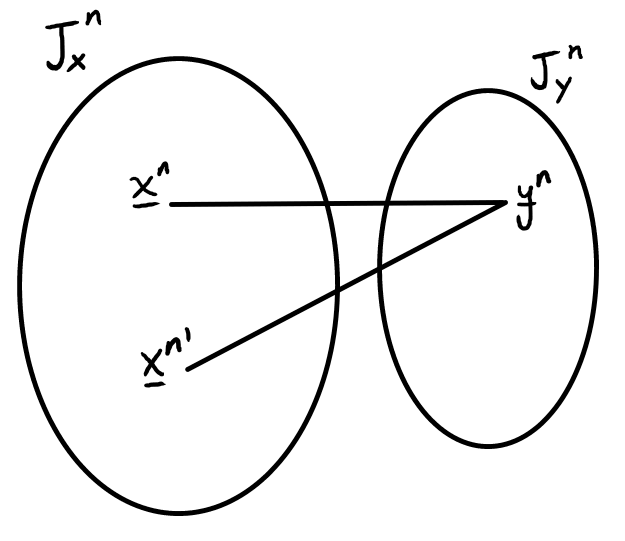
\includegraphics[width=0.35\textwidth]{2019/01/20190125_noisychannel1.png}
    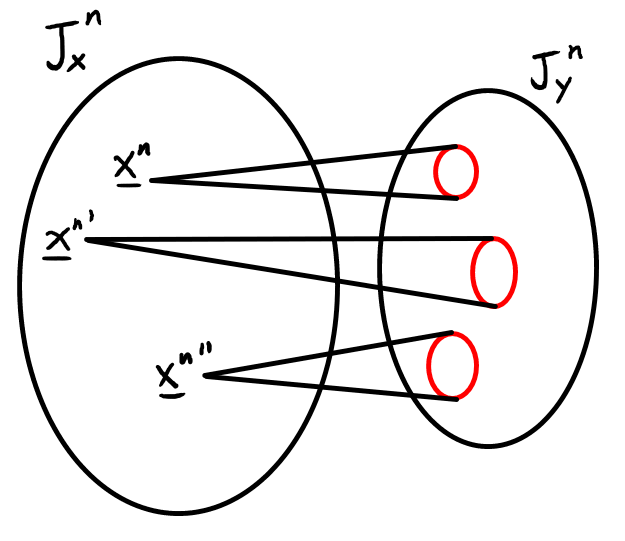
\includegraphics[width=0.35\textwidth]{2019/01/20190125_noisychannel2.png}
    \caption{In a noisy channel, it might be the case that multiple inputs map to the same output, as in the left set of ovals. Both $\underline{x}^n$ and $\underline{x}^n{}'$ have been mapped to the same $\underline{y}^n$ with some probability. However, Shannon tells us that certain codewords will be transmitted as disjoint regions (red ovals) after being sent through the channel, so those codewords can be reliably decoded after transmission.}
    \label{fig:noisychannel}
\end{figure}

We won't do the full proof of the theorem today, but we can introduce the setup. Suppose Alice has a message $[M]=\set{1,2,\ldots, M}$ she would like to send to Bob. She has a noisy channel $\mathcal{N}:J_X \to J_Y$ with some transition probabilities $p(\underline y^{n}| \underline x^{n})$.

%encoding-decoding Tikz figure
\begin{center}
    \begin{tikzpicture}[scale=2, node distance = 2.5cm]
        %make nodes
        \node [] (start) {};
        \node [block, right of=start] (encoding) {$\mathcal{E}_n$};
        \node [block, right of=encoding] (channel) {$\mathcal{N}$};
        \node [block, right of=channel] (decoding) {$\mathcal{D}_n$};
        \node [right of=decoding] (end) {};
        
        %make lines
        \path [line] (start) -- node[below] {$m\in M$} (encoding);
        \path [line] (encoding) -- node[below] {$x_m$} (channel);
        \path [line] (channel) -- node[below] {$y_m$} (decoding);
        \path [line] (decoding) -- node[below] {$m'$} (end);
    \end{tikzpicture}
\end{center}

\begin{enumerate}
    \item First, Alice can choose an encoding scheme $\mathcal{E}_n:[M]\to J_X^n$ where $\forall m\in [M], \mathcal{E}_n(m)=\underline x^{(n)} \in J_X^n$.
    \item She then sends her message through the channel $\mathcal{N}^{(n)}:x^{(n)}\to y^{(n)}$, producing some transmitted messages $y^{(n)}$ with some given probabilities.
    \item Bob receives the message and performs the decoding with $\mathcal{D}_n$ to get some decoded message $\mathcal{D}_n(\mathcal{N}^{(n)}(\mathcal{E}_n(M)))=m'$.
\end{enumerate}

Thus the \term{maximum probability of error} is
\begin{equation}
    \max{m\in [M]} P(\mathcal{D}_n(\mathcal{N}^{(n)}(\mathcal{E}_n(M))) \neq m) = p(\mathcal{E}_n,\mathcal{D}_n).
\end{equation}
We say that the \term{rate} is the number of the bits of the message transmitted per use of the channel. That is,
\begin{equation}
    R= \frac{\log M}{n}
\end{equation}
since $M \approx 2^{\lfloor nR \rfloor}.$

\begin{defn}
    We say that a rate is $R$ is \term{achievable} if there exists a sequence $(\mathcal{E}_n, \mathcal{D}_n)$ with $M=2^{nR}$ such that
    \begin{equation}
        \lim_{n\to \infty} p(\mathcal{E}_n,\mathcal{D}_n)= 0,
    \end{equation}
    i.e. the maximum probability of error tends to zero as $n$ goes to $\infty$.
\end{defn}

We make one final definition for today.
\begin{defn}
    The \term{channel capacity} is defined to be
    \begin{equation}
        C(\mathcal{N})=\sup \set{R: R\text{ is an achievable rate}},
    \end{equation}
    the maximum achievable rate for a channel.
\end{defn}

\subsection*{Non-lectured: m.b.s.c encoding}

For Example \ref{exm:mbsc}, we were asked to consider a binary channel $N$ with error probability $p$. That is, if we give it an input $x\in \set{0,1}$, we get an output $N(x)=y\in \set{0,1}$ such that $p(N(x)\neq x)=p$.

We came up with the following encoding scheme: send $0\mapsto 000$ and $1\mapsto 111$. To decode, we simply take a majority vote, e.g. $010$ was ``probably'' $000$, so the original message was $0$. Now how much better can we do with this redundancy? Let's consider the possible inputs, how they would be encoded, and how often they would be correct.

Suppose we want to send $0\mapsto 000$.
\begin{itemize}
    \item With probability $(1-p)^3$, none of the three bits are flipped and we get $000$ as the output. The process succeeds.
    \item With probability $3\times p(1-p)^2$, exactly one of the three bits is flipped. (The factor of $3$ comes from the fact that we could have flipped any of the three.) We still succeed.
    \item If two or three bits are flipped, we definitely fail.
\end{itemize}
By the symmetry of the problem, the success and failure probabilities are the same for $1\mapsto 111$.

Let's add this up to get the total success probability:
\begin{equation}
    (1-p)^3+3p(1-p)^2=(1+2p)(1-p)^2.
\end{equation}
When $p=1/2$, the success probability of our scheme is
\begin{equation}
    (1+2p)(1-p)^2=(2)(1/2)^2=1/2.
\end{equation}
We can nicely visualize this with the following graphic:
\begin{center}
    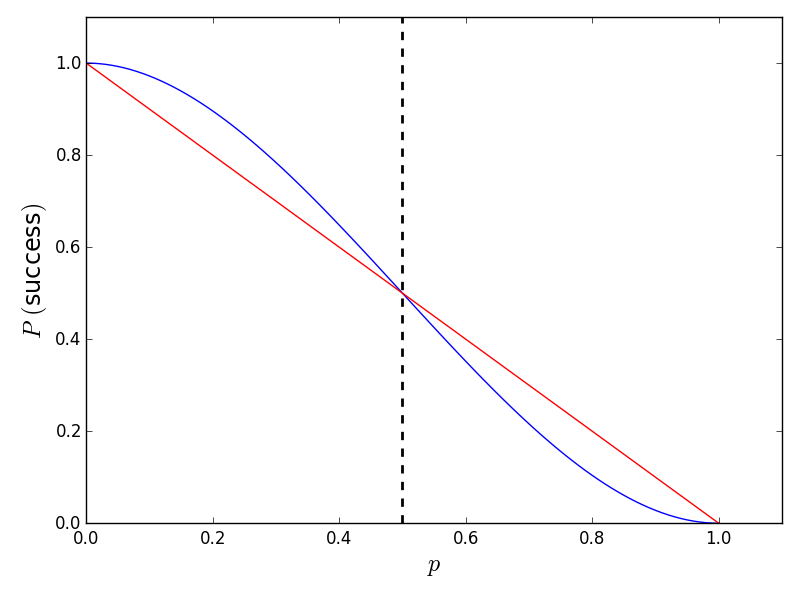
\includegraphics[width=0.5\textwidth]{2019/01/20190125_redundancy.png}
\end{center}
Here, the curved blue line is our three-bit scheme and the red line is the single-bit success probability $1-p$. For completeness, we can explicitly show that the crossover points occur when $P(\text{three bits})-P(\text{one bit})=(1+2p)(1-p)^2-(1-p)=0.$ Rewriting, we have $(1-p)(1-2p)p=0$, which clearly has zeroes at $p=0,1/2,1$. If we now take a derivative, we see that $\frac{d}{dp}\paren{P(\text{three bits})-P(\text{one bit})}|_{p=1/2}=1-6(1/2)+6(1/2)^2=-1/2,$ so $P(\text{three bits})>P(\text{one bit})$ for $p<1/2$.